\documentclass{article}
\usepackage[utf8]{inputenc}
\title{Report on the Multi-User-MISO Simulation System Design}
\author{Zhan Zhang}
\date{October 2016}

\usepackage{graphicx}
\usepackage[margin=0.5in]{geometry}


\begin{document}

\maketitle

\section{Introduction}
Currently, the multi-antenna technologies have been widely used in the modern communication system standards.
Therefore building up software simulation platforms for multi-antenna communication systems have received much attention.
This report introduces the design of a simulation platform for
the multi-user-multi-input-single-output (MU-MISO) communication system.
Zero-forcing technology is applied for beam-forming and two different
power allocation algorithms are implemented and performance evaluations are conducted based on them.

\section{System Model}
\subsection{Overview}
In this simulation platform, the communication system transmits signals via multiple transmission antennas to support multiple users.
Each user is assigned with a single receive antenna. The scenario is modelled in Figure 1.
\begin{figure}[ht]
\centering
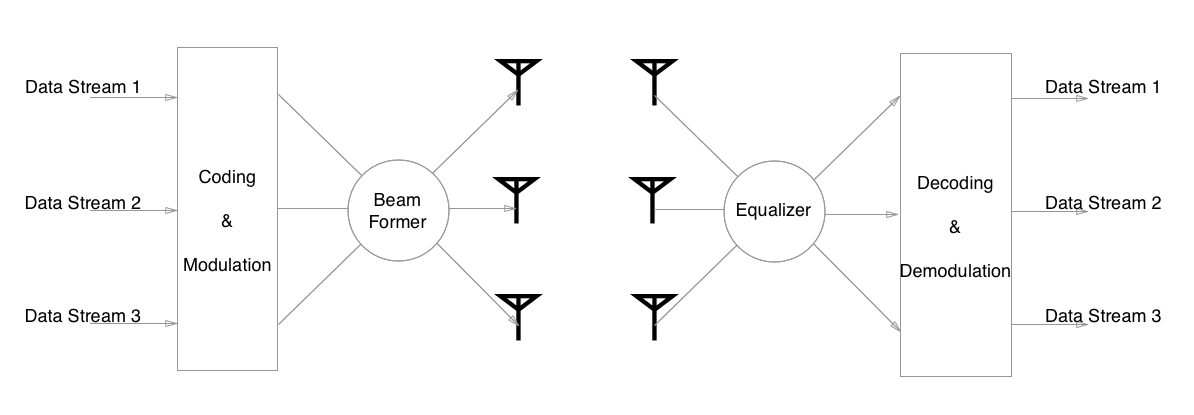
\includegraphics[scale=0.18]{Scenario.png}
\caption{The Scenario Model}
\label{fig:Scenario}
\end{figure}

The channel would be firstly simulated and the beamformer is calculated correspondingly.
Signal-to-Interference-and-Noise-Ratio for each user is calculated from the channel and the beam former to determine the modulation and coding scheme.
A data stream of a block length is then generate for each user for simulated transmission.
The system diagram is shown in figure 2.
\begin{figure}[ht]
\centering
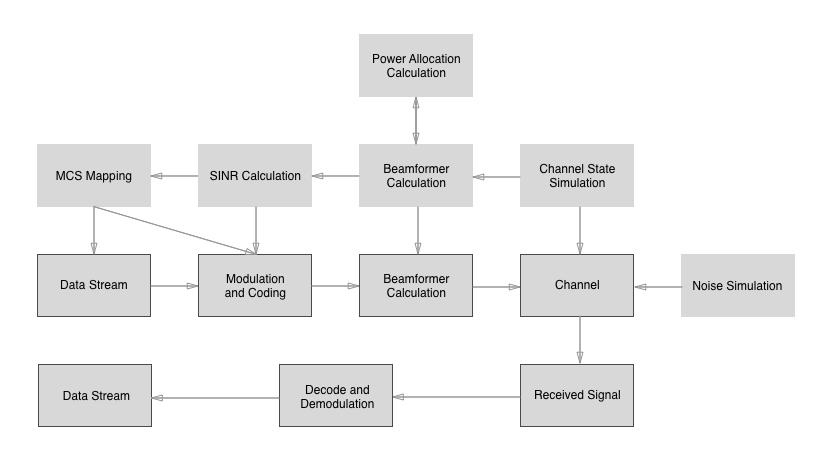
\includegraphics[scale=0.35]{SystemDia.png}
\caption{The System Diagram}
\label{fig:SystemDia}
\end{figure}
\subsection{Channel Simulation}
The channel is simulated as a complex matrix to include different paths.
The row vector in the matrix is the net channel for a single user and the column vector is the net channel for each transmitting antenna.
Assume the number of users to be $N_U$ and the number of transmitting antennas to be $N_T$, the matrix is produced of size $N_U * N_T$:
$$ \textbf{H} = randn(N_U,N_T) + j*randn(N_U,N_T)$$
The channel noise is simulated as random streams for users and then scaled to specific power level.
Assume the length of the signal to be T and the noise power to be $\sigma^2$, the noise matrix becomes:
$$
\textbf{v} = \frac{randn(T,N_U)+j*randn(T,N_U)}{\sqrt2}
$$
$$
\textbf{n} = \textbf{v}*\sigma
$$
\subsection{Beam Former and Power Allocation}
In this system, zero-forcing is employed for beam forming.
The beam former is calculated as the pseudo-inverse of the channel matrix to eliminate the inter-user-interference.
$$
\textbf{W} = \textbf{H}^H*(\textbf{H}*\textbf{H}^H)^{-1}
$$
A single column vector from $W$ is the beam former for single user.

The beam former is rescaled to fulfill the power constraint of the antennas. Two power allocation algorithms (Normalized and Water Filling) are implemented in this simulation system.
The power constraint of each antenna is set to be 1 for simplicity.
\subsubsection{Equal Power Scaling Allocation Scheme}
In the normalized scheme, the beam former matrix is normalized by its Frobenius Norm or the square root of the trace of $H*H^H$:
$$
\textbf{W} = \frac{\textbf{W}}{norm(\textbf{W}, 'fro')}
$$
\begin{center}or\end{center}
$$
\textbf{W} = \frac{\textbf{W}}{\sqrt{trace(\textbf{H}*\textbf{H}^H)}}   \hspace{1cm}(Equivalent)
$$
\subsubsection{Water Filling Scheme}
The water filling scheme is targeted to reach a maximum net data rate.
$$
\max \sum_{n=1}^{N_U} log(1+p_n)
$$
with the limitation of
$$\sum_{n=1}^{N_U} p_n \leq 1$$
Iterative division method is applied to find the value of $p$ to maximize the achievable rate.

\subsection{Signal Simulation}
\subsubsection{SINR Calculation}
With the channel \textbf{H} and the beam former \textbf{W} obtained, the SINR for each user is calculated to determine the modulation and coding scheme of the transmission.
The SINR for a single user is:
$$
SINR = \frac{\textbf{H}(User)*\textbf{W}(User)}{\sum_{n=1,n\ne User}^{N_U} \textbf{H}(User)*\textbf{W}(n)+\sigma}
$$
And convert it into decimal scale:
$$SINR(dB) = 10*log_10(SINR)$$
\subsubsection{Signal Generation}
According to the preset relationship, the SINR is mapped to certain CQI index then to MCS index.
The modulation and coding scheme is then determined.

As the block length ($L_{block}$) of the data bit is fixed for specific MCS, data stream of power 1 of the fixed length is generated for each user:
$$DataBits = logical(randi(2,1,L_{block})-1)$$
The data streams would then go through the corresponding modulator and the coder to form the signals(matrix $s$) for transmission.
\subsection{Beam Forming and Transmission}
The signals would be pre-coded by the beam former into signal (matrix $x$). This signal would be transmitted at the antennas.
$$x = W*s$$
x would be transmitted through the channel H and reach the receiving antenna.
The received signal would be:
$$y = H*x+n$$
The signal y is demodulated, decoded and detected back to the data streams.

\section{Performance Evaluation}
The detected data streams are compared to the original ones and check if there is any error. The blocks successfully transmitted is counted to the total through put.
The achievable rate is calculated from the SINR values:
$$AcRate = F*Bandwidth*log_2(1+SINR)$$
\begin{center}(F is the system loss of the OFDM)\end{center}
The performance comparison between the two power allocation schemes is shown in figure 3 (2-user-2-input system) .


\begin{figure}[ht]
\centering
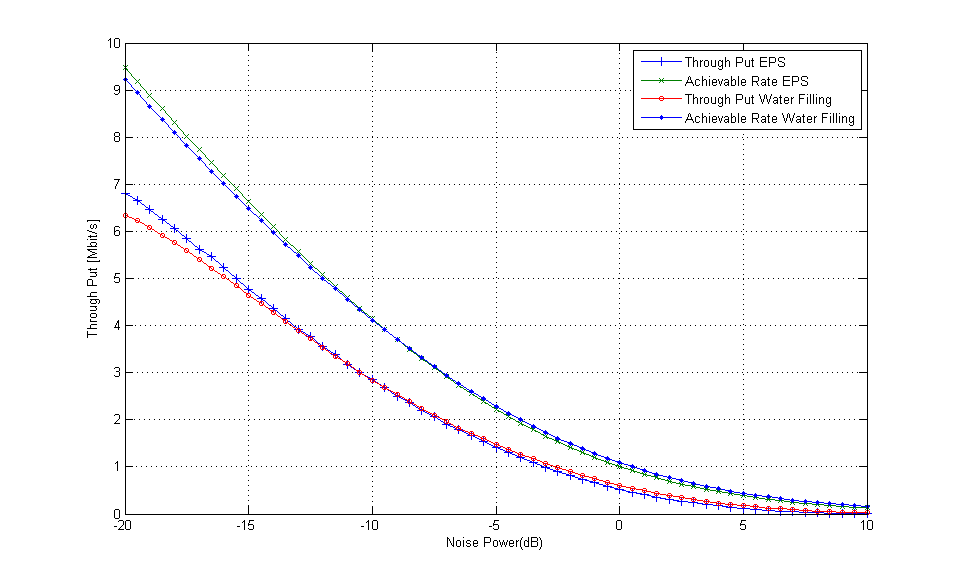
\includegraphics[scale=0.45]{WFvsEPS.png}
\caption{Water Filling vs EPS Comparison}
\label{fig:MUSOvsSISO}
\end{figure}
The waterfilling power allocation method performs better in net through put with high noise power.

The EPS method outperforms the waterfilling method when the noise power is low. This should be caused by the limitation of maximum transmit rate of the modulation and coding schemes.

The performance of the Single-Input-Single-Output(SISO) system is shown in figure 4. The performance is much boosted for the multi-antenna system comparing to the SISO system.
\begin{figure}[ht]
\centering
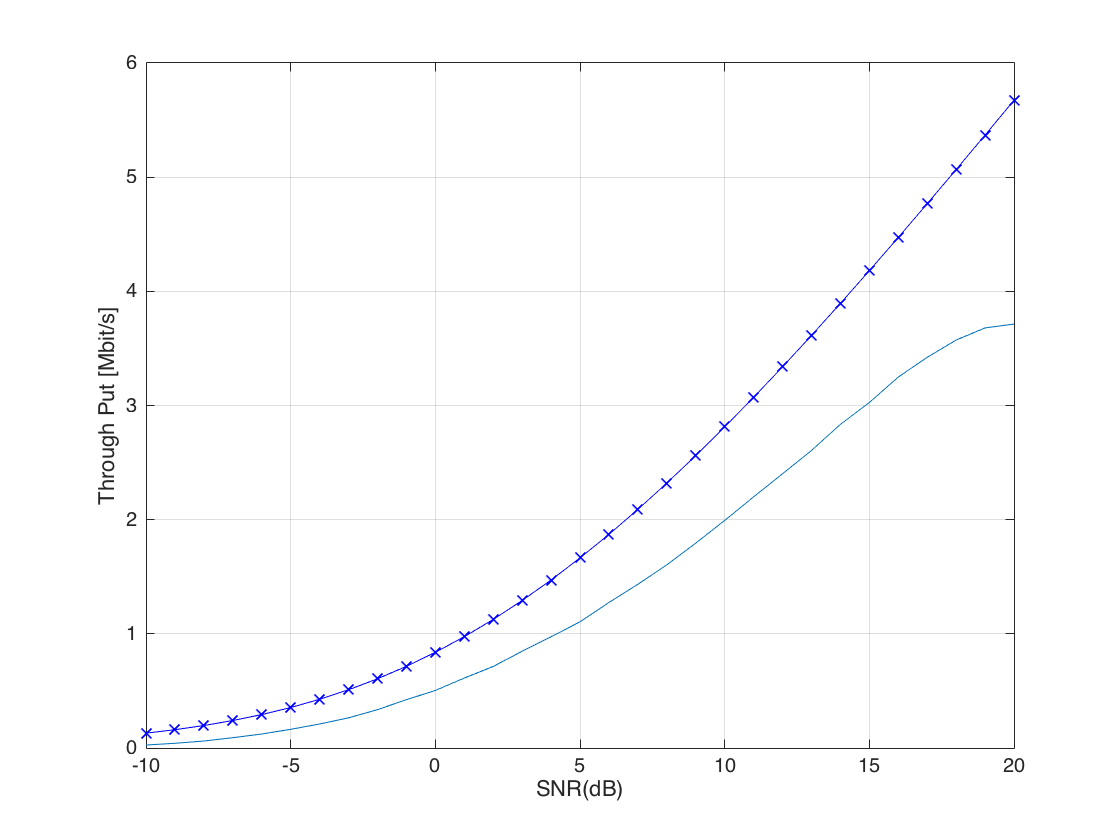
\includegraphics[scale=0.25]{FadingSISO.png}
\caption{SISO Performance}
\label{fig:WFvsEPS}
\end{figure}


\section{Conclusion}
The multi-antenna communication system have a much better net through put performance than the single antenna system.
The multi-antenna technology would be replacing the SISO system in modern communication systems to achieve better performances.

The water filling algorithm outperforms the EPS scheme at high noise power but loses the advantage at low noise power.
The constraint should be further researched and developed to overcome the problem.

\end{document}
